%\documentclass[11pt]{amsart}
\documentclass{article}
\usepackage{geometry}                % See geometry.pdf to learn the layout options. There are lots.
\geometry{letterpaper}                   % ... or a4paper or a5paper or ... 
%\geometry{landscape}                % Activate for for rotated page geometry
%\usepackage[parfill]{parskip}    % Activate to begin paragraphs with an empty line rather than an indent
\usepackage{graphicx}
\usepackage{amssymb}
\usepackage{epstopdf}
\usepackage{hyperref}
\DeclareGraphicsRule{.tif}{png}{.png}{`convert #1 `dirname #1`/`basename #1 .tif`.png}

\usepackage{mathtools}			%Creating an absolute value symbol a la http://tex.stackexchange.com/questions/43008/absolute-value-symbols
\DeclarePairedDelimiter\abs{\lvert}{\rvert}
\DeclarePairedDelimiter\norm{\lVert}{\rVert}
\makeatletter
\let\oldabs\abs
\def\abs{\@ifstar{\oldabs}{\oldabs*}}
\let\oldnorm\norm
\def\norm{\@ifstar{\oldnorm}{\oldnorm*}}
\makeatother


\title{The \textit{Atlas of Variability} Code Package and How to Use It}
\author{Kevin Schwarzwald}

%%%%%%%%%%%%%%%%%%%%%%%%%%%%%%%%%%%%%%%%%%%%%%%%%%%%%%%%%%%%%%%%%%
\begin{document}
\maketitle

\tableofcontents

\section*{0. Introduction}
The \textit{Atlas of Variability} Code Package was developed as part of the ``Atlas of Variability'' climate statistics project and is designed to allow for a quick, standardized analysis of the variability characteristics of climate model output. It is a series of Matlab functions and auxiliary programs that take NetCDF files and spit out results from spectral density analysis and basic distribution characteristics, and present them in several useful visualizations. 

Throughout this guide, \texttt{code input}, \texttt{function names} and \texttt{filenames} will be written in equal-spaced font, while \textbf{variables} will be written in bold. 

The code is written in MATLAB, and is based on the creation of standardized \texttt{.mat} files from the Raw NetCDF data. This procedure allows added code simplicity at the price of slower loading speeds, and it is suggested that future versions of this code allow support for keeping data in NetCDF format. 

Output is generally in \texttt{.mat} format for data and \texttt{.eps} and \texttt{.png} format for images. These are defaults that are simple to change (in the code itself) if desired.

The code package assumes one major set of calculations for each variable-data frequency-model-experiment(-run) combination. This procedure was sufficient for the large inter-model comparison done for the ``Atlas of Variability," but may cause problems if analyses of the same time series in multiple temporal chunks or analyses of different runs of the same individual model are desired. The code package is slowly being updated to allow for a more robust treatment of at least multiple runs per model, but a better treatment of different temporal chunks would require a change in filename standards for maps and ratio data (the pure output of the variability calculations is largely unaffected, since it uses the full original filename convention with only simplifying the dates into years). This is of course not an insurmountable obstacle by any means, and the user is encouraged to go down that path if the code package has not been sufficiently generalized at the time of use. 

Furthermore, the code makes several assumptions and simplifications. Generally, the default settings of the code assume calendars with 365-day years, and the pre-processing functions accordingly remove the 366th day of leap years to ensure compliance. This does not mean that the rest of the code cannot handle calendars with leap years or 360 days etc., but rather defaults must likely be changed or at least carefully considered to ensure the results are exactly what are desired (for example, one of the default `frequency bands' for daily data spans 30 - 365 days, which makes climatological sense in a 365-day calendar, but not in a 360-day calendar). Additionally, the code package is primarily set up to deal with time series chunks beginning on January 1st and ending on December 31st of any year. Though sub-annual (seasonal) analysis tools are included, the pre-processed time series, for filename simplicity, are expected to span integer multiples of years. 

Finally, filename conventions are based on CMIP5 defaults. The pre-processing code expects raw NetCDF files of a certain filename format, and does calculations based on values in certain positions in those filenames. See more details below. 

In general, users of this code package are expected to know their way around MATLAB (i.e.\ `do you know what the differences between a cell array, a struct, and a numerical array are?') and have a basic understanding of the NetCDF file structure. Every function has a detailed header description that often includes use examples and can be accessed by typing \texttt{help [function name]} into Matlab. 

For any questions, comments, concerns, complaints, etc., feel free to contact the author (Kevin Schwarzwald, kschwarzwald@uchicago.edu). 

\begin{figure}[h]
\caption{Function List}
\begin{center}
\begin{tabular}{l c | p{3.5in}}
Function Name&Type&Description\\ \hline
\texttt{various\_defaults}&Aux&Set file saving and processing defaults\\ 
\texttt{Saves}&Pre-processing&Convert NetCDF files into \texttt{.mat} files\\ 
\texttt{var\_chars}&Aux&Access variable-frequency information\\
\texttt{name\_chars}&Aux&Access individual file information\\ 
\texttt{Variability}&Variability&Calculate frequency band contributions to variability\\
\texttt{Variability\_seasons}&Variability&Calculate intra-/inter-seasonal variability\\
\texttt{Variability\_ci}&Variability&Get confidence intervals on variability changes\\
\texttt{load\_stddevs}&Aux&Load files, file subsets, and characteristics of variability data\\
\texttt{load\_means}&Aux&Load files, file subsets, and characteristics of mean data\\
\texttt{Maps\_stddev\_ci}&Mapping&Map changes in variability\\ 
\texttt{Maps\_pi\_flat}&Mapping&Map diagnostics of a variable\\
\texttt{Plots\_Log\_Panel\_prod}&Plotting& \\
\texttt{data\_colormap}&Aux&Assign colors to matrix elements\\
\texttt{clip\_lat}&Aux&Get indices of pixels within a latitude range\\
\texttt{clip\_region}&Aux&Get indices of pixels within a geographic region\\
\texttt{clip\_ci}&Aux&Get indices of pixels with non-significant variability changes\\
\texttt{clip\_minval}&Aux&Get indices of pixels above a certain value\\
\texttt{clip\_maxval}&Aux&Get indices of pixels below a certain value\\
\end{tabular}
\end{center}
\end{figure}


\section{Raw Data Processing} %% RAW DATA PROCESSING
\subsection{Setting Processing and Saving Defaults}\label{func:various_defaults.m}
All saving and processing defaults are stored in the file \texttt{various\_defaults.mat} and set by running the function \texttt{various\_defaults.m}. This program and file controls the directories for storing code, raw data, processed data, seasonal data, figures, and grid area weights. These must be set to the desired paths before running any other function in this package. These directories do not necessarily need to be different from another. NOTE: the code assumes that data is stored in model-specific subfolders of the relevant directories set by \texttt{various\_defaults.mat}. For example, raw NetCDF data for CCSM4 should be saved in the directory \texttt{[raw\_data\_dir]/CCSM4/}, with \texttt{[raw\_data\_dir]} set by \texttt{various\_defaults.m}. Please check the function header itself for a full list of which directories imply subdirectories. 

\texttt{various\_defaults.mat} also sets the default frequency bands calculated by \texttt{Variability.m} (see Section \ref{sec:var}). Finally, \texttt{various\_defaults.mat} sets model and experiment name conversions for display purposes (the filename versions of many experiment and model name are different from the human-readable names) and some auxiliary defaults useful for annotations. See the header of the file (\texttt{help various\_defaults} with it on the path) for more detailed descriptions.

\subsection{File Convention}
All functions beyond the pre-processing / saving functions assume the raw data is stored in a specific standardized (\texttt{.mat}) format in the \texttt{[raw\_data\_dir]/[model\_name]/} set by \texttt{various\_defaults.mat} run above, with the filenaming convention: 

\begin{equation}
\begin{split}
\texttt{filename} = \text{[file variable identifier]\_}&\text{[data frequency]\_[model]\_[experiment]\_}\\
&\text{[run]\_[start year]-[end year]\_DATA.mat}
\end{split}
\end{equation}

\begin{description}
\item [file variable identifier] shorthand variable name, e.g.\ \texttt{pr} for precipitation
\item [data frequency] month, day, etc., using CMIP5 conventions (\_Amon/\_Lmon/\_Omon for month, for whatever reason)
\item [model] model name in UNIX-safe character convention (so CSIRO Mk3.6.0 becomes CSIRO-Mk3-6-0)
\item [experiment] experiment / forcing profile, e.g.\ RCP8.5
\item [run] run ID (in CMIP5, [r\#i\#p\#] for run number, iteration, and microphysics; for non-CMIP5, can be anything)
\item [start year-end year] e.g.\ 2070-2099
\end{description}
and the following component parts: 
\begin{description}
\item [lat] latitude, either in vector \texttt{[}$m\times 1$ \texttt{double]} or array / grid (\texttt{[}$n\times m$ \texttt{double]} array) format
\item [lon] longitude, either in vector \texttt{[}$n\times 1$ \texttt{double]} or array / grid (\texttt{[}$n\times m$ \texttt{double]} array) format
\item [lat\_bnds] (optional) latitude bounds, with one additional dimension of size 2 compared to the latitude variable, giving the latitude vertices of each pixel
\item [lon\_bnds] (optional) longitude bounds, with one additional dimension of size 2 compared to the longitude variable, giving the longitude vertices of each pixel
\item [Raw] \texttt{[}$n\times m\times t$ \texttt{double]} array of data for one variable-frequency-model-experiment-run-timeframe combination, for number of longitude steps $n$, latitude steps $m$, and time steps $t$. \textbf{Raw} should always be 3-dimensional. 4-dimensional variables (such as pressure-delimited wind speed) should be split up by level in the 4th dimension into individual 3-dimensional files. 
\end{description}

The file naming convention is based on the conventions developed for the CMIP5 project, as are the variable and unit conventions. 

In general, the filename format above is used for most \textit{calculated} data files as well, with only the suffix changed (for example, a file with variability output would substitute \texttt{\_sqrtPower.mat} for \texttt{\_DATA.mat}).

\subsubsection{File Format}
In general, files should be stored as version 7.3 (HDF5, partial variable loading possible) with version 6 files (for compatibility with programs such as $R$ - the package \textit{R.matlab} can't deal with HDF5 files) saved separately if needed, and with the suffix \texttt{\_DATA\_v6.mat}. 

\subsubsection{File Saving Order}
Files should generally be saved in ascending order of variable size, meaning almost always \textbf{lat}, \textbf{lon}, (\textbf{lat\_bnds}, \textbf{lon\_bnds},) and \textbf{Raw}. This format allows for quicker loading of the geographic grid variables due to the way MATLAB compresses files in their newest file formats (accessing later variables requires some decompression of the previous variables).

\subsubsection{File Variable Identifiers}
For most variables, the file variable identifier should be modeled on the CMIP5 defaults (see the CMIP5 standard output (\href{cmip-pcmdi.llnl.gov/cmip5/docs/standard_output.pdf}{\underline{link}})). The most notable exception is 4-dimensional variables, such as pressure-delimited cloud or wind cover (\textbf{cl} and \textbf{ua}/\textbf{va} in CMIP5 format). In these cases, it is suggested to find a descriptive level-based identifier, for example \textbf{cllow} for low cloud cover or \textbf{ua850} for 850mb zonal wind velocity. 

\subsection{Saving Procedure} 
The \textit{Atlas of Variability} Code Package includes one program designed to process CMIP5 NetCDF data into the \texttt{\_DATA.mat} format, \texttt{Saves.m}. Given a \texttt{[var\_idx]} representing a variable and frequency in addition to a model, \texttt{Saves.m} looks into the \texttt{[raw\_data\_dir]} from \texttt{various\_defaults.m} to find one or more NetCDF files, and collates/clips them into a \texttt{.mat} file in the above convention of the desired length (by default, 30 years; see the function header for options on changing what chunk is extracted and saved). 

Daily / sub-daily data should generally be stored \textit{without leap years}! \texttt{Saves.m} does this automatically by removing the 366th day of leap years in gregorian / julian / proleptic gregorian calendars. 

\section{General Function Form} %% GENERAL FUNCTION FORM
Most non-auxiliary functions in this code package use a similar input concept. In general, these functions are called 
\begin{equation}
([\text{output}]) = \texttt{function}([\text{var\_idx}],[\text{model}],\dots)
\end{equation}

\begin{description}
\item [var\_idx] a row index or vector of row indices corresponding to a specific variable - data frequency combination(s) in the file \texttt{Varnames.csv} (see below)
\item [model] model name or cell array of model names in UNIX-safe character convention (so CSIRO-Mk3.6.0 becomes CSIRO-Mk3-6-0)
\end{description}

\subsection{Varnames.csv and How to Set Variable Name Conventions}\label{func:Varnames.csv}
The code package receives information about variable makeup from the text file \texttt{Varnames.csv}. Each row is one variable - data frequency combination (e.g.\ \texttt{pr\_day\_} $\equiv$ daily precipitation). Different programs in the code package will treat data differently based on the frequency (whether to remove leap years, how to calculate confidence intervals, etc.). The rest of the columns are purely used in graphing and displays. In accessing a row in the document, functions access standardized long names, units, and data types (ratio, interval, temp, etc., for choosing appropriate colorscales and colorbars in plotting) in addition to the shorthands for variable name and frequency used in filenames. This information is accessed in the code package using the function \texttt{var\_chars.m}. . 

The \textbf{var\_idx} mentioned above and called in most programs is simply the row index of the \texttt{Varnames.csv} file corresponding to the desired combination of variable and frequency. If desired, this procedure can be used to also differentiate between any of the graphing/display columns (i.e.\ have two columns for daily precipitation, but one with SI units ($kgm^2/s$) and one with meteorological units (like cm/s)). In this case, inserting the different row indices as \textbf{var\_idx} in programs will ensure that the resultant output displays the desired units. 

Support for variables can be added by simply adding a row, and information can be changed by editing the relevant element. Every row should include the information below (by column header):\begin{description}
\item [filevar] CMIP5 variable shorthand
\item [filevarFN] database variable shorthand (may be different from CMIP5, for example \textbf{ua850} for 850mb zonal wind velocity)
\item [freq] data frequency, following the CMIP5 standard (which means \_Amon, \_Lmon, etc.) and adding underscores before and after for filename processing purposes
\item [vardesc] variable long name, used in figure captions, etc.
\item [units] data and standard deviation units, surrounded by parentheses and a space (to counteract a graphics glitch in MATLAB text renderers)
\item [varunits] variance units (data units squared), in the same format
\item [clim\_type] data type deciding colorbar limits and colors - either \textbf{ratio} (greyscale), \textbf{interval} (blue to white/grey to red centered at 0), \textbf{percent} (greyscale, limits of [0, 100]), or \textbf{temp} (blue to white/grey to red, centered at 273)
\item [id] row number for easier reference
\end{description}

Though much of this data is theoretically accessible through the original NetCDF files, the idea behind a standardized variable `dictionary' is to make sure variable names and units are kept constant between climate projects that may use different conventions for all of these.

If a future version of this code package were to switch entirely to keeping data as NetCDF files, the information contained in \texttt{Varnames.csv} could be saved in the NetCDF header, with \textbf{[variable ID \#]} being replaced in program input by a variable name and data frequency combination. 

\subsection{Common Function Flags and Input Conventions}
Though I encourage you to refer to the header of each function for an exhaustive list of function flags and program run modifications (by typing \texttt{help [function name]} into the MATLAB console), a few flags are general across the code package and are worth enumerating here:

\begin{description}
\item [`testing'] adds the suffix \texttt{\_TEST} to the output filename(s)
\item [`experiments'] sets the experiment runs processed, in cell array format (e.g.\ \texttt{\{rcp85,piControl\}}, must be written as in filenames; different display names, for example RCP8.5 instead of rcp85, are supported through changing the \textbf{expArray\_disp} array in \texttt{various\_defaults.m})). Some code, such as \texttt{Maps\_stddev\_ci.m} or \texttt{SpectralRatios.m}, requires multiple experiment inputs in a specific order, please see function headers for exact requirements. 
\end{description}

\section{Calculating Variability} %% CALCULATING VARIABILITY
\subsection{Calculating Frequency Contributions to Variability}
\label{sec:var}\label{func:Variability.m}
The core purpose of this program package is to calculate the frequency-separated variability of an arbitrary climatic variable; in other words, the portion of the standard deviation contributed to by patterns within certain frequencies. This is done through the following process (a mathier description is found in Appendix [X]):

\begin{enumerate}
\item Detrending: a simple linear trend is removed from the time series (spectral density analysis requires stationarity)
\item Deseasonalization: the seasonal component of variability is removed by subtracting out a 12-harmonic least-squares fit
\item Spectral Density Calculation: a power spectrum is calculated from the resultant time series
\item Spectral Density Integration: the standard deviation is calculated by taking the square root of the integrated spectral density between the desired frequencies
\end{enumerate}

This process is executed through the function \texttt{Variability.m} (see the function header for a complete description). \texttt{Variability.m} takes in a \texttt{\_DATA.mat} file and outputs two files, with suffixes \texttt{\_LocalMeans.mat} and \texttt{\_sqrtPower.mat}. The former simply contains \textbf{lat}, \textbf{lon}, and a variable \textbf{LocalMeans}, an $[n\times m]$ array of the mean value of each grid point in the \texttt{\_DATA.mat} file over the relevant time period. The latter contains \textbf{lat}, \textbf{lon}, and a struct \textbf{StdDevs} that contains the calculated variability data in addition to the mean data already saved in \texttt{\_LocalMeans.mat}. The structure of \textbf{StdDevs} is as follows: 
\begin{description}
\item [StdDevs.Name] \texttt{\{`< 5 days',`5 - 30 days',\dots,`all frequenices'\}} (long name of frequency band, used in descriptions and graph titles)
\item [StdDevs.ID] \texttt{\{`HF',`MF',\dots,`Full'\}} (short identifier of frequency band, used in function input)
\item [StdDevs.Size] \texttt{\{[0,5],[5,30],\dots,[0 Inf]\}} (period limits of each frequency band, for reference)
\item [StdDevs.Data] \texttt{\{[}$n\times m$ \texttt{double],\dots\}} (standard deviation portion contributed by the frequency band)
\end{description}

The struct \textbf{StdDevs} also includes entries for the local mean values (as in \texttt{\_LocalMeans.mat} above) stored with \textbf{ID} = \texttt{`mean'} and the standard deviation stored with \textbf{ID} = \texttt{`std'}. The standard deviation is usually not exactly equal to the \texttt{`Full'} / all frequency band due to estimation precision in the spectral density calculation. Both \texttt{`std'} and \texttt{`mean'} are stored with \textbf{Size} = \texttt{[ ]} (an empty array). 

\subsection{Calculating Seasonal Variability}
\label{func:Variability_seasons.m}

\subsection{Calculating Variability Ratios}
\label{func:SpectralRatios.m}
For a slight simplification in manual examination of variability change data, the code package allows for the creation of extra files that store the ratio of frequency-separated variability between two experiments (these files are also necessary to run \texttt{Maps\_stddev\_ci.m}). This process occurs through the program \texttt{SpectralRatios.m}. The function is called as normal, with an important input to remember:
\begin{equation}
\texttt{SpectralRatios}([\text{variable ID \#}],[\text{model}],(\text{`experiments'},\{exp_2,exp_1\}),\dots)
\end{equation}
$exp_2$ and $exp_1$ are the two experiments between which the ratio should be calculated. Specifically, the ratio will be calculated as $\frac{exp_2}{exp_1}$ and is by default set as $exp_2=$ \texttt{rcp85} and $exp_1=$ \texttt{piControl}.

The output file has the suffix \texttt{\_SpectralRatios.m} and the same structure as the \texttt{\_sqrtPower.m} file explained above, with the only difference being the name of the struct (\textbf{StdDevsRatio} instead of \textbf{StdDevs}). Importantly, the output filename no longer has the [\texttt{year}] field - in the current structure of the file system only one ratio file can be stored per run and experiment combination. To ensure that the SpectralRatios file is created from time series with the same length, the program cycles through \texttt{\_sqrtPower.m} files to find a matching pair (with warnings being thrown if equal length time series could not be found for both experiments). 

\subsection{Getting Confidence Intervals on Variability Changes}
\label{sec:var_ci}\label{func:Variability_CI.m}
\texttt{Variability\_CI.m} allows the generation of confidence intervals on ratios of frequency-separated variability (and any other quantity saved in the \textbf{StdDevs} structs, such as mean or standard deviation). In absence of a large ensemble of runs of the same model, this is done using a boostrap methodology (see Appendix [XX] for derivation). NOTE: currently this procedure only supports daily data! Similar to \texttt{SpectralRatios.m}, \texttt{Variability\_CI.m} requires the input of two experiments: 
\begin{equation}
\texttt{Variability\_CI}([\text{variable ID \#}],[\text{model}],(\text{`experiments'},\{exp_2,exp_1\}),\dots)
\end{equation}

The output file has the suffix \texttt{\_StdDevCI.mat} and has the same variables as \texttt{\_StdDevsRatio.mat} files above (\textbf{lat}, \textbf{lon}, \textbf{StdDevsRatio}) with the addition of a variable \textbf{file\_params} with the experiments, runs, and start/end years of the \texttt{\_DATA.mat} files used in the program run.\footnote{THIS SHOULD PROBABLY BE ADDED AS A FUNCTIONALITY TO \texttt{SpectralRatios.m} AS WELL}

The variable \textbf{StdDevsRatio} has the fields (the first four are equivalent to \textbf{StdDevs} and \textbf{StdDevsRatio} above):
\begin{description}
\item [StdDevs.Name] \texttt{\{`< 5 days',`5 - 30 days',\dots,`all frequencies'\}} (long name of frequency band, used in descriptions and graph titles)
\item [StdDevs.ID] \texttt{\{`HF',`MF',\dots,`Full'\}} (short identifier of frequency band, used in function input)
\item [StdDevs.Size] \texttt{\{[0,5],[5,30],\dots,[0 Inf]\}} (period limits of each frequency band, for reference)
\item [StdDevs.Data] \texttt{\{[}$n\times m$ \texttt{double],\dots\}} (standard deviation portion contributed by the frequency band)
\item [std\_runs] \texttt{\{[}$n\times m$ \texttt{double],\dots\}} the local standard deviation $\sigma$ across bootstrap runs of the ratio of variabilities; confidence intervals are determined as $2\sigma$ from the calculated ratio
\item [lon\_ciidx] \texttt{\{[}$k\times 1$ \texttt{double],\dots\}} longitude indices of pixels in which the ratio of variabilities is not meaningfully different from 1 (the confidence interval includes 1)
\item [lat\_ciidx] \texttt{\{[}$k\times 1$ \texttt{double],\dots\}} latitude indices of pixels in which the ratio of variabilities is not meaningfully different from 1 (the confidence interval includes 1)
\end{description}


\section{Mapping Results} %% MAPPING RESULTS
\label{func:Maps_stddev_ci.m}
The code package includes some basic mapping tools. The most robust, and most used in the ``Atlas of Variability'' Project is \texttt{Maps\_stddev\_ci.m}, which produces a map / up to 6 subplotted maps of the change in variability between two experiments of a variable - frequency - model combination, and can hash out pixels without a meaningful change in variability, as calculated in \texttt{Variability\_CI.m}. It requires a previously calculated \texttt{\_SpectralRatios.mat} file for the experiments to be compared, and, if a marking of pixels without meaningful changes is desired, a previously calculated \texttt{\_StdDevsCI.mat} file.

Beyond the general functional form (as always, check the function header through \texttt{help Maps\_stddev\_ci} for all flags and details), I would like to point out two specific function flags:
\begin{description}
\item [`show\_freqs'] a cell array of the form \texttt{\{`HF',`MF',\dots,`Full'\}} (with 1 - 6 cells), including the \textbf{ID}/short data identifier of the desired frequency band / quantity to be graphed
\item [`plot\_method'] followed by either \texttt{`pcolorm'} or \texttt{`polygon'}. The former is the default, and uses the matlab function \texttt{pcolorm} to produce a geographic checkboard/pseudocolor plot. However, the pcolorm paradigm plots data at vertices, and so removes a row and column from each side (see \href{http://www.mathworks.com/matlabcentral/fileexchange/50706-offsets-and-missing-data-via-pcolor-and-surf?focused=3873981&tab=example}{\underline{here}} for details). The option \texttt{`polygon'} instead graphs each individual pixel as a filled polygon, solving this issue at the expense of computational efficiency (plotting and saving individual polygons results in a significant increase in processing time, and is therefore generally suggested to be used for production figures only). An added benefit of the \texttt{`polgyon'} option is the ability to more accurately show the shape of pixels in non-rectangular grids. Pixel edges are rectangular and taken from the \textbf{lat\_bnds} and \textbf{lon\_bnds} variables in a NetCDF file from the same model with the same lat/lon grid as the data. In other words, it searches the raw data folder's (set in \texttt{various\_defaults.m}) relevant model subset directory for a NetCDF file with the same lat/lon grid and the variables \textbf{lat\_bnds} and \textbf{lon\_bnds}. If this is not found, latitude and longitude bounds are inferred as being halfway between pixel coordinates, and a warning is thrown. 
\end{description}

\section{Graphing Results} %% GRAPHING RESULTS
\label{func:Plots_Log_Panel_prod.m}

\section{Auxiliary Functions} %% AUXILIARY FUNCTIONS
\subsection{Loading calculated data}
The filenames used in the CMIP5 models and throughout this code package are admittedly a bit of a mouthful. Here's a few functions designed to make loading data a bit simpler and more pleasant.
\subsubsection{Loading data from \texttt{\_sqrtPower.mat} files}
\texttt{load\_stddevs.m} allows for the direct loading of the struct \textbf{StdDevs}, the lat/lon grid, or even subsets of the \textbf{StdDevs} struct (such as the IDs contained within it, etc.). The basic function call is as follows:
\begin{equation}
\textbf{[StdDevs,lat,lon]} = \texttt{load\_stddevs([var\_idx],[model],[experiment],([season]),\dots)}
\end{equation}
To make loading such data even easier, \texttt{[var\_idx]} can be replaced by the CMIP5 shorthands for variable and frequency, for example: \texttt{load\_stddevs(`pr',`day',\dots)}. To get the filename that the function is loading (to verify timeframe, etc.), add the flag \texttt{`filename'}. To get properties within the \textbf{StdDevs} struct, use the flag \texttt{`property',[field name]}. 

\subsubsection{Loading data from \texttt{\_LocalMeans.mat} files}
\texttt{load\_means.m} allows for the direct loading of the file LocalMeans or the lat/lon grid. The basic function call is as follows:
\begin{equation}
\textbf{[LocalMeans,lat,lon]} = \texttt{load\_means([var\_idx],[model],[experiment],([season]),\dots)}
\end{equation}
The data in \textbf{LocalMeans} is also found as \textbf{ID} $=$ \texttt{mean} in \textbf{StdDevs} above, but this allows a more direct loading of the mean values of a time series. 

\subsection{Subsetting data by region, value, etc.}
The following are several functions designed to give linear indices of pixels that fulfill a certain geographic, numerical, or meaningfulness criteria. In general, these \texttt{clip\_*.m} files follow a basic input/output paradigm:
\begin{equation}
\begin{aligned}
\textbf{idx\_clipped} &= \texttt{clip\_*(\dots)} \\
\textbf{idx\_unclipped} &= \texttt{clip\_*(\dots,idxs,\dots)}
\end{aligned}
\end{equation}
These two forms allow for both getting the linear indices of pixels that match the criteria determined through \texttt{clip\_*} (\textbf{idx\_clipped}) or the linear indices of pixels that do not match the same criteria (\textbf{idx\_unclipped}). In the latter case, an existing vector of `unclipped' indices \textbf{idxs} should be added (can be an empty vector, see individual function headers for a more detailed description). 

\subsubsection{Clipping data by region}
\begin{figure}[h] %% Regions Map
\centering
	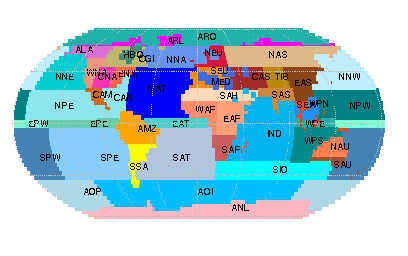
\includegraphics[width=19pc,angle=0]{RegionsMap.pdf}\\
	\caption{Map of regions used in \texttt{clip\_region.m}}\label{fig:regions_map}
\end{figure}

\texttt{clip\_region.m} allows the return of (linear) indices of an array of points lying within a geographic region or multiple regions. The basic function call is:
\begin{equation}
\textbf{idx\_clipped} = \texttt{clip\_region(region\_id,model,lat,lon)}
\end{equation}
The information needed to set region boundaries is found in the file \texttt{regions.mat} in the basic code folder. This file contains a struct \textbf{Regions}, containing a lat/lon bounding box (the fields \textbf{lon\_min}, \textbf{lon\_max},\textbf{lat\_min}, \textbf{lat\_max}), whether the region is land or ocean (the field \textbf{Type} = \texttt{`LAND'}, \texttt{`OCEAN'}, or \texttt{`LAND'}), and a short ID and long name for the region (the fields \textbf{ID} and \textbf{Name}). Each `region' is defined as points lying within a lat/lon bounding box, and potentially limited to just land or ocean pixels. More regions can be added by editing the struct \textbf{Regions}. The existing regions are those used by \cite{castruccio_statistical_2013} (see Figure \ref{fig:regions_map}). 

The lat/lon grid does \textit{not} have to be global. Indices will be returned based on the inputted lat/lon grid.

\textbf{region\_id} in the function input above can either be the field \textbf{ID} of the relevant region or its index in the struct \textbf{Regions}. Multiple regions can also be inputted simultaneously in a cell array \texttt{\{region\_id$_1$,region\_id$_2$,\dots\}}. In this case the resultant output is based on the union of pixels in the inputted regions.  

The model needs to be inputted (in normal string format, i.e.\ \texttt{`CSIRO-Mk3-6-0'}) because of the need for a surface-land fraction grid to determine land/ocean pixels in a specific model. If at least one of the desired regions is land or ocean only, the program then looks in the raw data folder for the model for a file \texttt{sftlf*.mat} with a matching lat/lon grid as inputted in the variables \textbf{lat} and \textbf{lon}. No such action if the region(s) inputted are not land- or ocean-specific (and the \texttt{sftlf*.mat} file is then not needed). The latitude and longitude grid does not have to cover the whole globe! As long as the lat/lon grid can be found within the \texttt{sftlf*.mat} grid, the correct indices will be output, with an error if the subset was not found. 

\subsubsection{Clipping data by latitude band}
\texttt{clip\_lat.m} allows the return of (linear) indices of an array of points lying between two latitude values (absolute, by default). The basic function call is:
\begin{equation}
\textbf{idx\_clipped} = \texttt{clip\_lat(lat\_min,lat\_max,lat,lon)}
\end{equation}
By default, the indices of points are given that lie between the absolute value of \texttt{lat\_min} and \texttt{lat\_max}; in other words, for both the Northern and Southern hemispheres. To just return indices in a specific hemisphere, the flag 
\begin{equation}
\textbf{idx\_clipped} = \texttt{clip\_lat(\dots,`hemisphere',[`NH'/`SH'],\dots)}
\end{equation}
can be used. As an additional output, the exact latitudes used can be shown in a struct, see the specific function documentation for more information. 

\subsubsection{Clipping variability data by significance}
\texttt{clip\_ci.m} allows the return of (linear) indices of points determined to have an insignificant change in the variable between experiments, as calculated through \texttt{Variability\_CI.m} (see Section \ref{func:Variability_CI.m}). The basic function call is: 
\begin{equation}
\textbf{idx\_clipped} = \texttt{clip\_ci(var\_idx,model,expArray)}
\end{equation}
This clip requires a relevant \texttt{\_StdDevCI.mat} file calculated through \texttt{Variability\_CI.m} to function.  


\section{Additional Functions / Files} %% ADDITIONAL FUNCTIONS / FILES
\subsection{Background Functions}

\subsection{Third Party/Community Functions}
A few functions are taken from the MATLAB community. 

\begin{figure}[h]
\caption{Third-Party Function List}
\begin{center}
\begin{tabular}{l p{1.5in} | p{3in}}
Function Name&Type&Description\\ \hline
\texttt{ds2nfu}&Plotting&Converts from data units to normalized figure units for placing objects onto plots\\
\texttt{structfind}&Aux&Gets index of a struct based on matching a specific field\\
\texttt{rgb}&Returns RGB triplet for CSS3 colors\\
\texttt{wraptext}&Aux&Wraps output text\\ 
\end{tabular}
\end{center}
\end{figure}


\section{Typical Code Run} %% TYPICAL CODE RUN (show the Basic File Saves or whatever it's called)
The following shows an example code run from start to finish analyzing the relationship between changes in daily precipitation variability and mean in the model CSIRO Mk3.6.0 between RCP8.5 and pre-industrial control and between RCP8.5 and historical runs. The \texttt{`experiments'} calls aren't strictly necessary (except for RCP8.5 - historical comparisons) since they just represent the default function behavior, but are included for reference.
\begin{enumerate}
\item set raw / processed / output data directories in \texttt{various\_defaults.m} (Section \ref{func:various_defaults.m}); add the model to the \textbf{modelArray\_disp} variable to accommodate the model name (`CSIRO-Mk3-6-0' in the filesystem, `CSIRO Mk3.6.0' in figure captions); add the experiments to the \textbf{expArray\_disp} variable to accommodate experiment names (`rcp85' / `historical' / `piControl in the filesystem, `RCP8.5' / `Historical' / `PI Control' in figure captions)
\item download \texttt{pr\_day\_CSIRO-Mk3-6-0\_rcp85*.nc}, \texttt{pr\_day\_CSIRO-Mk3-6-0\_historical*.nc}, and \texttt{pr\_day\_CSIRO-Mk3-6-0\_piControl*.nc} files from ESGF, DKRZ, or your other favorite climate model data repository into the raw data directory set above
\item run \texttt{Saves(5,\{`CSIRO-Mk3-6-0'\},`experiments',\{`rcp85',`historical',`piControl'\})} for daily precipitation row index 5 (from \texttt{Varnames.csv}, Section \ref{func:Varnames.csv}) to pre-process data into 30-year \texttt{*\_DATA.mat} files and to remove leap days
\item run \texttt{Variability(5,\{`CSIRO-Mk3-6-0'\},`experiments',\{`rcp85',`historical',`piControl'\})} (Section \ref{func:Variability.m}) to calculate integrated spectral densities, means, and standard deviations
\item run \texttt{SpectralRatios(5,\{`CSIRO-Mk3-6-0'\},`experiments',\{`rcp85',`piControl'\})} and \texttt{SpectralRatios(5,\{`CSIRO-Mk3-6-0'\},`experiments',\{`rcp85',`historical'\})} (Section \ref{func:SpectralRatios.m}) to save variability ratios
\item run \texttt{Maps\_stddevs\_ci(5,\{`CSIRO-Mk3-6-0'\}, `experiments',\{`rcp85',`piControl'\},}\\ \texttt{`show\_freqs',\{`HF',`MF',`mean',`LF'\})} and \texttt{Maps\_stddevs\_ci(5,\{`CSIRO-Mk3-6-0'\}, \\`experiments',\{`rcp85',`historical'\}, `show\_freqs',\{`HF',`MF',`mean',`LF'\})} (Section \ref{func:Maps_stddev_ci.m}) to map the $<$ 5 day variability, 5 - 30 day variability, mean, and 30 - 365 day variability changes in daily precipitation between RCP8.5 and PI control and RCP8.5 and historical runs
\item run \texttt{Plots\_Log\_Panel\_prod(5, \{`CSIRO-Mk3-6-0'\}, `experiments', \{`rcp85',`piControl'\}, `show\_freqs', \{`LF',`XF'\}, `clip\_lat',30,55, `color\_by',`data', \{`piControl'\}, \{`mean'\}, `log10')} (Section \label{func:Plots_Log_Panel_prod.m}) to create a scatterplot of variability changes vs.\ mean changes for 30 - 365 day and $>$ 1 year variability (in 2 subplots) in the mid-latitudes ($\abs{30^\circ-55^\circ}$), colored by the base-10 log of pre-industrial mean precipitation
\end{enumerate}

%%%%%%%%%%%%%%%%%%%%%%%%%%%%%%%%%%%%%%%%%%%%%
\bibliographystyle{ieeetr}
\bibliography{paper_cites_mkii.bib}

%%%%%%%%%%%%%%%%%%%%%%%%%%%%%%%%%%%%%%%%%%%%%
\appendix
\section{Conventions, Names, etc. Typically Found in Model-World}
\subsection{Typical Model Experiments}
\subsubsection{Transient vs. Equilibrated Model Runs}


\subsubsection{The Representative Concentration Pathways (RCPs)}


\subsection{Typical Model Technical Details}

\subsubsection{Some Model Grids}
\begin{description}
\item [Basic Rectangular Lat/Lon Grids] the simplest grid - the earth is split up into a $lat\times lon$ grid with 1D vector \textbf{lat} and \textbf{lon} vectors. 
\item [Gaussian Grids] usually named [letter][number]. Naming conventions differ; NCAR uses T\#\#, with the number determining the spectral truncation (some explanation  \href{https://software.ecmwf.int/wiki/display/FCST/Relationship+between+spectral+truncation+and+grid+point+resolution}{\underline{here?}}). The grid is also rectangular, however latitudes are unequally spaced and defined by the Gaussian quadrature. No grid points at the poles. Typically the number of longitudes are twice that of latitudes. Can also be uniquely described by 1D \textbf{lat} and \textbf{lon} vectors. Gaussian grids allow for easier computation of integrals involved in the Fourier and Legendre transforms. 
\item [Orthogonal Curvilinear Grids] often used for ocean grids. Cannot be described by vectors in lat/lon space, \textbf{lat} and \textbf{lon} must be 2D arrays. Allows for a computationally efficient approach to grids with differing spatial scales. Based on a transformation from a rectangular grid. 
\end{description}

\subsubsection{Model Components}
%Add Knutti family tree, one of the images from the bubble diagrams of model components grouped by code size
See the Software Architecture of Climate Models. 
\begin{figure}[h]
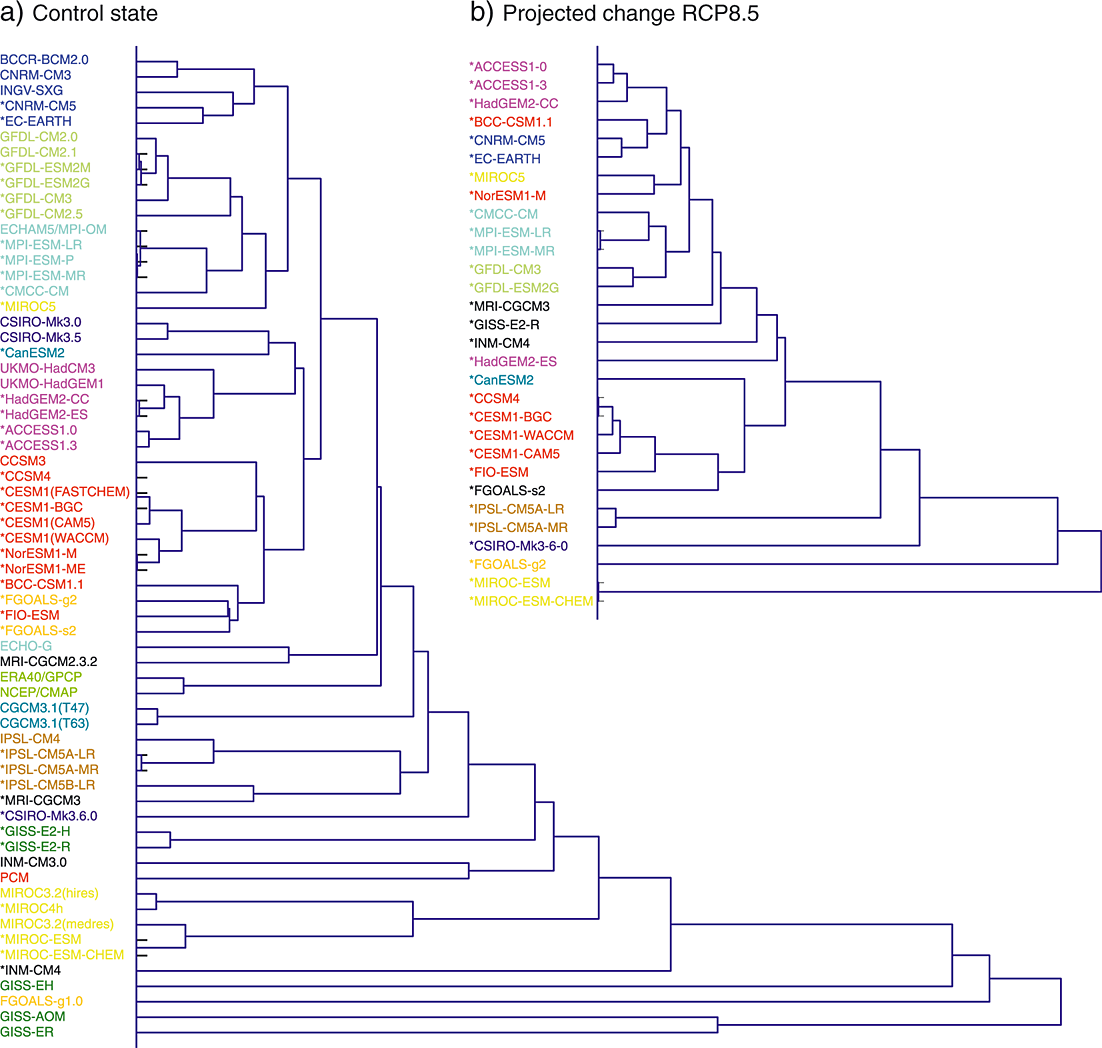
\includegraphics[width=\textwidth]{Knutti_family_tree.png}
\caption{Figure and following caption copied from \cite{knutti_climate_2013}: (a) The model ``family tree" from CMIP3 and CMIP5 (marked with asterisks) control climate plus observations (ERA40/GPCP and NCEP/CMAP), shown as a dendrogram (a hierarchical clustering of the pairwise distance matrix for temperature and precipitation fields, see text). Some of the models with obvious similarities in code or produced by the same institution are marked with the same color. Models appearing in the same branch are close, and similarity is larger the more to the left the branches separate (for a detailed description of the method, see Masson and Knutti [2011]). (b) Same but based on the predicted change in temperature and precipitation fields for the end of the 21st century in the RCP8.5 scenario relative to the control.}
\end{figure} 


\section{Math stuff}
High- (i.e.\ the pattern of rain showers) and low-frequency (i.e.\ droughts, extreme precipitation events) patterns of precipitation are affected by different climatological processes, and could therefore react differently to changes in temperature and gas concentrations in addition to having differing impacts on human society. To isolate changes in variability for different precipitation processes, we use spectral density analysis to study variability in different frequency `bands' by decomposing the time series for each model output pixel into it frequency components. To do so, we largely adapt the methodology introduced in \cite{leeds_simulation_2015} and \cite{klavans_influence_2016} based on integrations over power spectra.

Spectral density calculations assume stationarity in the underlying time series, so we first detrend the climatic data. We isolate non-seasonal variability by several data frequency-based deseasonalization methods. Finally, we calculate band-separated variability from power spectra. 
%Appendix deseasonalization math
\subsection{Detrending and Deseasonalization} %%% Detrending, Deseasonalization
\label{sec:detrend_deseas}
\subsubsection{Daily Data} %Daily Data
A classic decomposition of a time series $Y$ is as follows: 
\begin{equation}
\begin{aligned}\centering
Y &= X_ta + Y_c \\
Y &= m_t + s_t + Y_c \\ 
Y_c &= Y - m_t - s_t 
\end{aligned}\end{equation}
for trend $m_t$, seasonal component $s_t$ (with a known period), and a variability component $Y_c$. $m_t$ is either $0$ if the time series is already stationary (as it is with equilibrated CCSM3 runs) or is made to equal $0$ through subtracting a linear trend, leaving
\begin{equation}
Y_c = Y-s_t
\end{equation}
The seasonal component is then removed by fitting harmonic components using least squares. Given the least-squares process
\begin{equation}Y_c = Y-s_t\hat{\beta}\label{eq:deseas}\end{equation}
for 
$$\hat{\beta} = \frac{s'_ts_t}{s'_tY}$$
we fit
\begin{equation}
s_t = \left[1 \cos\left(\frac{2\pi}{365}\left[\begin{matrix}1 \\ \vdots \\ t\end{matrix}\right][1 \hdots \lambda]\right) \sin\left(\frac{2\pi}{365}\left[\begin{matrix}1 \\ \vdots \\ t\end{matrix}\right][1 \hdots \lambda]\right) \right]
\end{equation}
for length of (daily) time series $t$ and number of harmonics to be removed $\lambda$. In the general process for daily time series used in this project, $\lambda = 12$, and for 30-year time series, $t = 10950$. Subtracting $s_t\hat{\beta}$ from equation \ref{eq:deseas} above results in $Y_c$ now representing the detrended, deseasonalized, variable component of the time series, ready to be further analyzed. 

\subsubsection{Monthly Data} %Monthly Data
Monthly data was deseasonalized by taken the simple average of each month over the length of each time series and subtracting it from every data month. $Y_c$, the deseasonlized time series $Y$ over $T$ years, was constructed as follows: 
\begin{equation}
Y_c(y,m) = Y(y,m) - \frac{1}{T}\sum_{y=1}^T Y(y,m)
\end{equation}
for each month $m$ and year $y$.

\subsection{Spectral Analysis} %%% Spectral Analysis
\label{sec:spec_analysis}
%Appendix spectral analysis math
The autocorrelation function for a stationary process $x(t)$ with mean $\mu=0$ and variance $\sigma^2$ is given by
$$\begin{aligned}
R(\tau) &= \frac{1}{\sigma^2}E[(x_t-\mu)(x_{t+\tau}-\mu)] \\
R(\tau) &= \frac{1}{\sigma^2}E[x_tx_{t+\tau}] \end{aligned}$$
and is periodic at the same period as the original function $x(t)$. Peaks in $R(\tau)$ correspond to periodicites with frequencies $\tau$ - the autocorrelation function finds interior periodicites in the original time series. By the Wiener-Khinchin Theorem, the autocorrelation function makes a Fourier Pair with the power spectral density $S_{xx}(\omega)$ as follows: 
$$S_{xx}(\omega) = \int_{-\infty}^\infty R(\tau)e^{-i\omega \tau}d\tau$$
The absolute value of the Fourier Transform as a function of frequency gives the amount of that frequency that is present in the original function, in this case $R(\tau)$. Therefore the (infinite) sum of the Fourier transforms over a range of frequencies gives the contribution of those frequencies to the autocorrelation, which gives how strongly different frequency patterns show up in the time series. In other words, 
\begin{equation} \begin{aligned} \int_{\omega_1}^{\omega_2}S_{xx}(\omega)d\omega &= \frac{1}{T}\int_{\omega_1}^{\omega_2}\abs{\hat{x}(\omega)}^2d\omega \\
&= \text{contribution to power by }\omega\in[\omega_1,\omega_2]\label{eq:FT_power}\end{aligned}\end{equation}
Now, taking the sample variance of a discrete stationary time series $x$ of length $N$ with mean $\mu=0$,
$$ \begin{aligned}
\sigma^2 &\equiv \frac{1}{N}\sum^N_{i=1}(x_i-\mu)^2 \\ 
\sigma^2 &= \frac{1}{N}\sum^N_{i=1}(x_i)^2 \end{aligned}$$
and assuming an infinite time series ($N\rightarrow \infty$), we see that the variance of a time series is related to its average power $\bar{P}$ over the domain $[-T,T]$ through
$$\sigma^2 = \lim_{N\rightarrow\infty}\frac{1}{N}\sum^N_{i=1}(x_i)^2\rightarrow \lim_{T\rightarrow \infty}\frac{1}{2T}\int^T_{-T}x(t)^2dt = \bar{P}$$
Using Parceval's theorem, which states
$$\int_{-\infty}^{\infty}\abs{x(t)}^2dt = \int_{-\infty}^{\infty}\abs{\hat{x}(\omega)}^2d\omega$$
for the Fourier transform $\hat{x}(f)$ of $x(t)$, we can see that 
$$\frac{1}{2T}\int_{-\infty}^{\infty}\abs{\hat{x}(\omega)}^2d\omega = \frac{1}{T}\int_{0}^{\infty}\abs{\hat{x}(\omega)}^2d\omega= \sigma^2$$
Combining this expression with equation \ref{eq:FT_power} above, 
\begin{equation} 
\frac{1}{T}\int_{\omega_1}^{\omega_2}\abs{\hat{x}(\omega)}^2d\omega = \sigma^2\{\omega\in[\omega_1,\omega_2]\}
\end{equation}
with the standard deviation contained in those frequencies simply given by the square root of the expression, 
\begin{equation}
\sigma(\vec{\omega})\equiv\sigma\{\omega\in[\omega_1,\omega_2]\} = \sqrt{\frac{1}{T}\int_{\omega_1}^{\omega_2}\abs{\hat{x}(\omega)}^2d\omega}
\end{equation}
where we have used $\sigma(\vec{\omega})$ for ease of notation in the article text. 

\subsection{Bootstrap Procedure} %%% Bootstrap Procedure
\label{sec:bootstrap}
Given the time series representing precipitation at a single pixel for one experiment run spanning \textit{n} years, for each bootstrap run a new time series was created also spanning \textit{n} `years', but with each year starting at a random time step in the original time series. The years are allowed to `wrap-around', so if a randomly chosen start interval was less than a year from the end of the original time series, the counter continues at the start of the time series instead. For example, for a 30-year time series, a new time series was created using 30 randomly chosen start indices in the domain [1,10950] (10950 days in 30 years), counting up 365 days from each start index, and concatenating end-to-end. 

Variability contributed by different frequency bands were calculated as above for each run. Then, for each run, the ratio of future / past variability for each frequency band was taken. The standard deviation across runs for this ratio was taken for each frequency band. If the outputted final value of that ratio is within two standard deviations as so calculated of 1 (no change), then the change in variability for that pixel is not considered meaningful. 1200 runs are used by default. 

\section{Frequently Used Input Terms}

\begin{description}
\item [expArray] a cell array of ...
\item [log] (in a function header) logical 0/\texttt{false} or 1/\texttt{true}
\item [cell] (in a function header) a cell array of strings, numbers, etc.\ (e.g.\ \texttt{\{`rcp85',\dots\}})
\end{description}







\end{document}